% Chapter 3 KNN-LSTSVM

\chapter{ماشین بردار پیشتیبان دو قلو کمترین مربعات مبتنی بر نزدیک‌ترین همسایه }\label{ch:3}
\section{مقدمه}\label{sec:3:1}
نقطه ضعف بزرگ روش \lr{TSVM} و \lr{LS-TSVM} این است که این روش‌ها اطلاعات شباهت  بین نمونه‌های آموزشی را در نظر نمی‌گیرند. به عبارت دیگر، به تمام نمونه‌های آموزشی اهمیت یکسانی داده می‌شود. بطوریکه نمونه‌های نویزی و پرت دقت مدل خروجی را روی داده‌های جدید کاهش می‌دهد. روش \lr{WLTSVM} این نقطه ضعف مهم را حل کرده است. این روش با ساخت گراف نزدیک‌ترین همسایه، اطلاعات درون و برون کلاسی را در تابع هدف مسئله بهینه‌سازی لحاظ کرده است. بطوریکه به هر یک از نمونه‌های آموزشی وزن نسبت می‌دهد و همچنین نمونه‌های حاشیه‌ای هر کلاس را استخراج می‌کند.

روش \lr{WLTSVM} مانند \lr{TSVM} اصلی، دو مسئله بهینه‌سازی دوگان از نوع برنامه‌ریزی درجه دو حل می‌کند. بطوریکه آموزش روش \lr{WLTSVM} بر روی مجموعه داده‌های بزرگ کند و زمان‌بر خواهد بود. در این فصل، با گرفتن ایده از روش‌های \lr{LS-TSVM} و \lr{WLTSVM}، روش جدید ماشین بردار پشتیبان دو قلو کمترین مربعات مبتنی بر رویکرد نزدیک‌ترین همسایه (\lr{KNN-LSTSVM}) ارائه می‌شود \cite{mir2018}. روش پیشنهادی دارای مزایای زیر است:

\begin{itemize}[label=$\bullet$]
	\item روش پیشنهادی (\lr{KNN-LSTSVM})، مشابه روش \lr{WLTSVM} به طور کامل از اطلاعات شباهت بین نمونه‌ها استفاده می‌کند. بطوریکه با ساخت گراف نزدیک‌ترین همسایه اطلاعات درون و برون کلاسی را در مسئله بهینه‌سازی لحاظ می‌کند. به عبارت دیگر، به هر نمونه آموزشی بر اساس شمارش تعداد نزدیک‌ترین همسایه‌هایش وزن داده می‌شود. همچنین نمونه‌های حاشیه‌ای هر کلاس نیز مشخص می‌گردد.
	\item روش پیشنهادی مشابه روش \lr{LS-TSVM}، دو دستگاه معادلات خطی برای بدست آوردن مدل خروجی حل می‌کند. این مزیت روش پیشنهادی را به یک الگوریتم ساده با پیچیدگی محاسباتی کمتر از \lr{WLTSVM} تبدیل می‌کند. به طور کلی، روش \lr{KNN-LSTSVM} نیازی به الگوریتم‌های بهینه‌سازی برای حل مسائل دوگان ندارد.
	\item روش پیشنهادی برخلاف روش \lr{LS-TSVM} نسبت به نمونه‌های پرت حساسیت کمتری دارد. زیرا با استفاده از گراف نزدیک‌ترین همسایه به نمونه‌های پرت و نویزی ورن کمتری نسبت داده می‌شود. بنابراین مدل خروجی دقت بهتری خواهد داشت.
\end{itemize}

در ادامه این فصل، ابتدا نحوه ساخت ماتریس وزن‌ها از طریق گراف \lr{k} نزدیک‌ترین همسایه شرح داده می‌شود. سپس نسخه خطی و غیر خطی روش \lr{KNN-LSTSVM} توضیح داده شده است.

\section{ساخت ماتریس وزن‌ها}\label{sec:3:2}
ایده اصلی روش پیشنهادی (\lr{KNN-LSTSVM}) و \lr{WLTSVM} این است که به نمونه‌های با تراکم بیشتر وزن بیشتری بدهد و از کلاس مقابل نمونه‌های حاشیه‌ای را مشخص کند. به عبارت دیگر، ابرصفحه غیرموازی در روش \lr{KNN-LSTSVM} به نمونه‌های پرتراکم نزدیک‌تر است و از نمونه‌های حاشیه‌ای کلاس مقابل حداکثر فاصله را می‌گیرد. شکل \ref{fig:KNN-LSTSVM-LSTSVM} تفسیر هندسی روش \lr{LS-TSVM} و \lr{KNN-LSTSVM} را نشان می‌دهد.

\begin{figure}[!b]
	\centering
	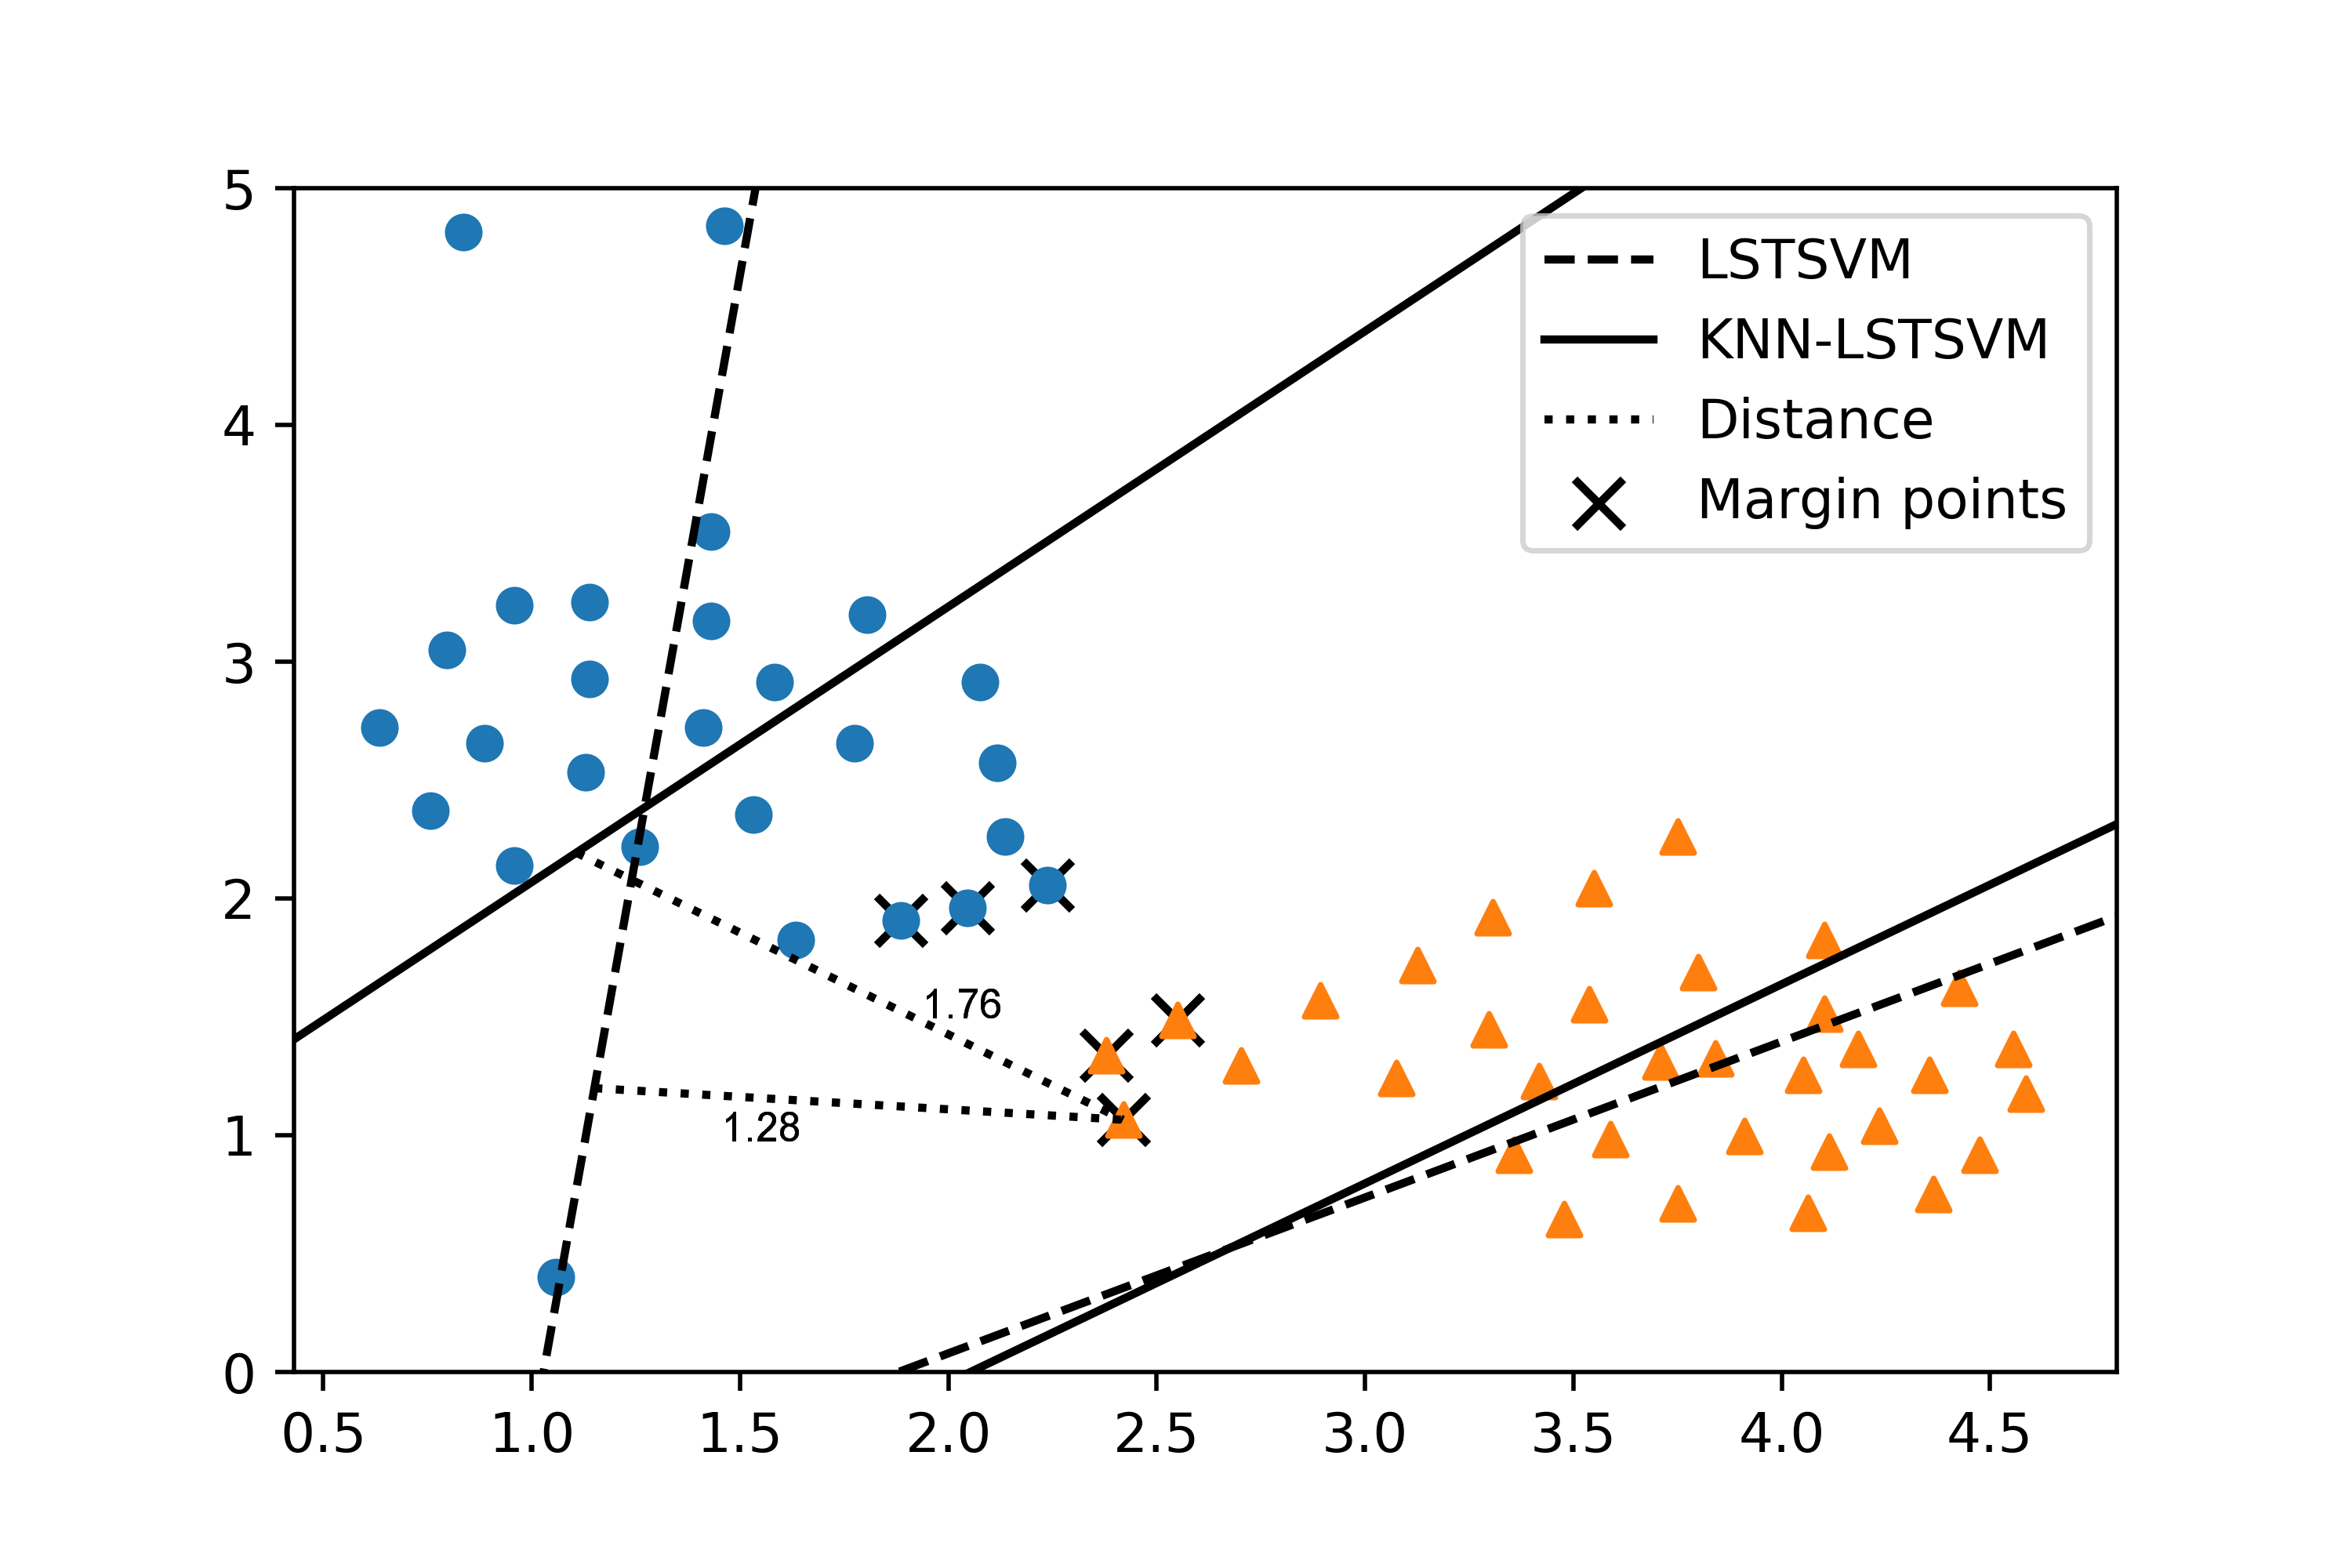
\includegraphics[scale=0.1]{KNN-LSTSVM-vs-LSTSVM}
	\caption{ تفسیر هندسی روش \lr{LS-TSVM} و \lr{KNN-LSTSVM}}
	\label{fig:KNN-LSTSVM-LSTSVM}
\end{figure}

همانطور که در شکل \ref{fig:KNN-LSTSVM-LSTSVM} مشخص شده است، ابرصفحه غیرموازی در \lr{LS-TSVM} به نمونه‌های پرت (کلاس دایره) بسیار نزدیک است. در حالی که روش پیشنهادی (\lr{KNN-LSTSVM}) از نمونه‌های پرت فاصله قابل توجه‌ای دارد و به نواحی پرتراکم نزدیک تر است. همچنین فاصله عمودی یک نمونه حاشیه‌ای از ابرصفحه هر دو روش در شکل ‏\ref{fig:KNN-LSTSVM-LSTSVM} محاسبه شده است. روش پیشنهادی از نمونه‌های حاشیه‌ای فاصله بیشتری دارد.

ابتدا گراف \lr{k} نزدیک‌ترین همسایه جهت بدست آوردن ماتریس وزن‌ها به صورت زیر تعریف می‌شود.
\begin{equation}\label{eq:63}
W_{ij} =
\begin{cases}
1, & \textrm{\lr{if }} x_i \in Nea\left(x_j\right)\textrm{\lr{ or }} x_j \in Nea\left(x_i\right),  \\
0, & \textrm{\lr{otherwise }}.
\end{cases}
\end{equation}

در رابطه \ref{eq:63}، مجموعه  شامل $k$ نزدیک‌ترین همسایه نمونه  $x_i$ است که در رابطه زیر تعریف شده است.
\begin{equation}\label{eq:64}
N(x_j) = \{x^1_j, x^2_j, \dots , x^k_j\}
\end{equation}

گراف $W$ به تنهایی نمی‌تواند تفکیک پذیری در داده‌ها را پیدا کند. در عوض یک گراف درون کلاسی  $W_{w,ij}$ و برون کلاسی   $W_{b,ij}$ ایجاد می‌شود تا به ترتیب فشردگی درون کلاسی\LTRfootnote{\lr{Intra-class compactness}}  و جداپذیری برون کلاسی\LTRfootnote{\lr{Inter-class separability}}  مشخص شود. ماتریس وزن $W_{w}$ و  $W_{b}$ به ترتیب در روابط \ref{eq:65} و \ref{eq:66} تعریف شده است.
\begin{equation}\label{eq:65}
W_{w,ij} =
\begin{cases}
1, & \textrm{\lr{if }} x_i \in N_w(x_j) \textrm{\lr{ or }} x_j \in N_w(x_i)  \\
0, & \textrm{\lr{otherwise }}.
\end{cases}
\end{equation}
\begin{equation}\label{eq:66}
W_{b,ij} =
\begin{cases}
1, & \textrm{\lr{if }} x_i \in N_b(x_j) \textrm{\lr{ or }} x_j \in N_b(x_i)  \\
0, & \textrm{\lr{otherwise}}.
\end{cases}
\end{equation}

در رابطه \ref{eq:65} و \ref{eq:66}، مجموعه $N_w(x_j)$ نشان‌دهنده $k$ نزدیک‌ترین همسایه نمونه $x_j$ از کلاس خودش و $N_b(x_j)$ مجموعه   شامل $k$ نزدیک‌ترین همسایه نمونه  $x_j$ از کلاس مقابل است. دو مجموعه $N_w(x_j)$ و $N_b(x_j)$ به ترتیب در روابط \ref{eq:67} و \ref{eq:68} تعریف شده‌اند.
\begin{align}
\label{eq:67}
\begin{split}
N_w\left(x_i\right) = \{x^j_i \mid l(x^j_i) = l(x_i), 1 \leq j \leq k \}
\end{split} \\
\label{eq:68}
\begin{split}
N_b\left(x_i\right) = \{x^j_i \mid l(x^j_i) \neq l(x_i), 1 \leq j \leq k \}
\end{split}
\end{align}

در رابطه \ref{eq:67} و \ref{eq:68}،  $l(x_i)$ نشان‌دهنده برچسب نمونه $x_i$ است. بدیهی است که  $N_w(x_i)\, \cap \, N_b(x_i) = \varnothing $ و  $N_w(x_i)\, \cup \, N_b(x_i) = N(x_i)$. فاصله بین هر کدام از نمونه‌های آموزشی توسط قاعده اقلیدس محاسبه می‌شود. به منظور پیدا کردن نمونه‌های حاشیه‌ای کلاس منفی، ماتریس وزن  $W_{b}$ به صورت زیر بازتعریف می‌شود.
\begin{equation}\label{eq:69}
f_{j} =
\begin{cases}
1, & \textrm{\lr{if }} \exists i, W_{b,ij} \neq 0  \\
0, & \textrm{\lr{otherwise}}.
\end{cases}
\end{equation}   

وزن هر کدام از نمونه‌های کلاس مثبت به صورت زیر محاسبه می‌شود.
\begin{equation}\label{eq:70}
{{d}_{j}}=~\underset{i=1}{\overset{{{m}_{1}}}{\mathop \sum }}\,{{W}_{w,~ij}}~,~j=1,2,\ldots ,~{{m}_{1}}
\end{equation}

در رابطه \ref{eq:70}، $d_j$  نشان‌دهنده وزن نمونه $x_j$ است. در اینجا تعداد همسایه‌ها با برچسب یکسان، وزن یک نمونه را مشخص می‌کند.

\section{نسخه خطی}\label{sec:2:3}
روش پیشنهادی مشابه روش \lr{WLTSVM}، دو ابرصفحه غیر موازی ایجاد می‌کند. بطوریکه هر کدام از این ابرصفحه‌ها به نمونه‌های پرتراکم نزدیک‌تر است و از نمونه‌های حاشیه‌ای کلاس مقابل حداکثر فاصله را دارد. با این حال روش پیشنهادی (\lr{KNN-LSTSVM})، مسائل اصلی روش \lr{WLTSVM} را تغییر می‌دهد. به این صورت که نامعادله در قید مسئله بهینه‌سازی به قید مساوی تغییر می‌یابد و همچنین متغیر لغزش به توان دو رسیده است.

راه حل دو مسئله اصلی تغییر یافته نیاز به حل کردن دو دستگاه معادلات خطی دارد. در حالی که در روش \lr{WLTSVM}، دو مسئله دوگان باید حل شود. مسئله اصلی تغییر یافته کلاس مثبت به صورت زیر تعریف می‌شود.
\begin{equation}\label{eq:71}
\begin{split}
\mathop{{ min}}\limits_{w_{(1)} ,b_{(1)}} \qquad & \frac{1}{2}{{(A{{w}^{\left( 1 \right)}}+e{{b}^{\left( 1 \right)}})}^{T}}D(A{{w}^{\left( 1 \right)}} +e{{b}^{\left( 1 \right)}}) +\frac{C}{2}{{y}^{T}}y \\
\textrm{\lr{s.t. }} \qquad & -F(B{{w}^{\left( 1 \right)}}+e{{b}^{\left( 1 \right)}})+y=Fe
\end{split}
\end{equation} 

 در رابطه \ref{eq:71}،  $D=diag(d_1,\dots,d_{m_{1}})$ نشان‌دهنده ماتریس وزن کلاس مثبت و $F=diag(f_1,\dots, f_{m_{2}})$ نشان دهنده نمونه‌های حاشیه‌ای کلاس منفی است. مقدار $f_j$ برابر با 0 یا 1 است و $d_i$ برزگتر یا مساوی با صفر است ($d_i \geq 0$).
 
 مزیت مهم مسئله اصلی \ref{eq:71} این است که که می‌توان قید مساوی را در آن در جایگذاری کرد. بنابراین تابع لاگرانژ مسئله اصلی \ref{eq:71} به صورت تعریف می‌شود.
\begin{equation}\label{eq:72}
 \mathop{{ min}}\limits_{w_{(1)} ,b_{(1)}} L = \quad \frac{1}{2}{{\left\| D(A{{w}^{(1)}}+{{e}}{{b}^{(1)}}) \right\|}^{2}} +{\frac{C}{2}}{{\left\|F( B{{w}^{(1)}}+{{e}}{{b}^{(1)}})+F{e} \right\|}^{2}}
\end{equation}

با گرفتن مشتق‌گیری جزئی از رابطه \ref{eq:72} نسبت به  $w^{(1)}$ و $b^{(1)}$  خواهیم داشت:
 \begin{align}
 \label{eq:73}
 \begin{split}
 \frac{\partial L}{\partial w^{(1)}} &= {{A}^{T}}D(A{{w}^{\left(1\right)}}+e{{b}^{\left( 1 \right)}} ) + C{{B}^{T}}F(B{{w}^{\left( 1 \right)}}+e{{b}^{\left( 1 \right)}}+Fe)=0e
 \end{split}\\
 \label{eq:74}
 \begin{split}
 \frac{\partial L}{\partial b^{(1)}} &= {{e}^{T}}D(A{{w}^{\left( 1 \right)}}+e{{b}^{\left( 1 \right)}}) + C{{e}^{T}}F(B{{w}^{\left( 1 \right)}}+e{{b}^{\left( 1 \right)}}+e)=0
 \end{split}
 \end{align}
 
 در ادامه با ترکیب کردن روابط \ref{eq:73} و \ref{eq:74} دستگاه معادلات خطی زیر بدست می‌آید.
 \begin{equation}\label{eq:75}
 \left[ \begin{matrix}
 {{B}^{T}}FB\, & {{B}^{T}}Fe  \\
 {{e}^{T}}FB\, & {{e}^{T}}Fe  \\
 \end{matrix} \right]\left[ \begin{matrix}
 {{w}^{\left( 1 \right)}}  \\
 {{b}^{\left( 1 \right)}}  \\
 \end{matrix} \right]+\frac{1}{C}\left[ \begin{matrix}
 {{A}^{T}}DA\, & {{A}^{T}}De  \\
 {{e}^{T}}DA\, & {{e}^{T}}De  \\
 \end{matrix} \right]\left[ \begin{matrix}
 {{w}^{\left( 1 \right)}}  \\
 {{b}^{\left( 1 \right)}}  \\
 \end{matrix} \right] +\left[ \begin{matrix}
 {{B}^{T}}Fe  \\
 {{e}^{T}}Fe  \\
 \end{matrix} \right]=0e.
 \end{equation}
 \begin{equation}\label{eq:76}
 \left[ \begin{matrix}
 {{w}^{\left( 1 \right)}}  \\
 {{b}^{\left( 1 \right)}}  \\
 \end{matrix} \right]={{\left[ \begin{matrix}
 		{{B}^{T}}FB+~\frac{1}{C}{{A}^{T}}DA\, & {{B}^{T}}Fe+\frac{1}{C}{{A}^{T}}De\,  \\
 		{{e}^{T}}FB+~\frac{1}{C}{{e}^{T}}DA\, & {{e}^{T}}Fe+\frac{1}{C}{{e}^{T}}De\,  \\
 		\end{matrix} \right]}^{-1}} \times \left[ \begin{matrix}
 -{{B}^{T}}Fe  \\
 -{{e}^{T}}Fe  \\
 \end{matrix} \right]
 \end{equation}
 \begin{equation}\label{eq:77}
 \left[ \begin{matrix}
 {{w}^{\left( 1 \right)}}  \\
 {{b}^{\left( 1 \right)}}  \\
 \end{matrix} \right]={{\left[ \begin{matrix}
 		\left[ \begin{matrix}
 		{{B}^{T}}  \\
 		{{e}^{T}}  \\
 		\end{matrix} \right]F & \left[ \begin{matrix}
 		B & e  \\
 		\end{matrix} \right]+~\frac{1}{C}\left[ \begin{matrix}
 		{{A}^{T}}  \\
 		{{e}^{T}}  \\
 		\end{matrix} \right]D\left[ \begin{matrix}
 		A & e  \\
 		\end{matrix} \right]  \\
 		\end{matrix} \right]}^{-1}} \times \left[ \begin{matrix}
 \left[ \begin{matrix}
 -{{B}^{T}}  \\
 -{{e}^{T}}  \\
 \end{matrix} \right] & Fe  \\
 \end{matrix} \right]
 \end{equation}
 
با تعریف کردن ماتریس $H$ و $G$ به صورت $H=[A\text{ }e]$ و $G=[B\text{ }e]$، راه حل مسئله بهینه‌سازی \ref{eq:71} به صورت زیر تعریف می‌شود.
\begin{equation}\label{eq:78}
\left[ \begin{matrix}
{{w}^{\left( 1 \right)}}  \\
{{b}^{\left( 1 \right)}}  \\
\end{matrix} \right] = -{{({{G}^{T}}FG+\frac{1}{C}{{H}^{T}}DH)}^{-1}}{{G}^{T}}Fe
\end{equation}

مسئله اصلی تغییر یافته کلاس منفی به صورت زیر تعریف می‌شود.
\begin{equation}\label{eq:79}
\begin{split}
\mathop{{ min}}\limits_{w_{(2)} ,b_{(2)}} \qquad & \frac{1}{2}{{(B{{w}^{\left( 2 \right)}}+e{{b}^{\left( 2 \right)}})}^{T}}Q(B{{w}^{\left( 2 \right)}}+e{{b}^{\left( 2 \right)}})+\frac{C}{2}{{y}^{T}}y \\
\textrm{\lr{s.t. }} \qquad & P(A{{w}^{\left( 2 \right)}}+e{{b}^{\left( 2\right)}})+y=Pe
\end{split}
\end{equation}

در رابطه \ref{eq:79}،  $Q=diag(q_1,\dots,q_{m_{2}})$ نشان‌دهنده ماتریس وزن کلاس منفی و  $P=diag(p_1,\dots  ,p_{m_{1}})$ نشان‌دهنده نمونه‌های حاشیه‌ای کلاس مثبت است. مانند ماتریس $F$، مقدار $p_j$  برابر 0 یا 1 است.

راه حل مسئله اصلی \ref{eq:79} همانند کلاس مثبت با جایگذاری قید مساوی، گرفتن مشتق‌گیری جزئی به صورت زیر تعریف می‌شود.
\begin{equation}\label{eq:80}
\left[ \begin{matrix}
{{w}^{\left( 2 \right)}}  \\
{{b}^{\left( 2 \right)}}  \\
\end{matrix} \right] = {{({{H}^{T}}PH+\frac{1}{C}{{G}^{T}}QG)}^{-1}}{{H}^{T}}Pe
\end{equation}

راه حل‌های \ref{eq:78} و \ref{eq:80} شامل دو معکوس ماتریس با اندازه $(n+1)\times (n +1)$ است. بطوریکه $n$ بسیار کوچکتر از تعداد نمونه‌های کلاس مثبت و منفی می‌باشد. بنابراین سرعت یادگیری نسخه خطی روش \lr{KNN-LSTSVM} بسیار زیاد است.

تابع تصمیم نسخه خطی به صورت زیر تعریف می‌شود.
\begin{equation}\label{eq:81}
D(x_i) =
\begin{cases}
+1, & \textrm{\lr{if }} |{{x}^T}{{w}^{(1)}}+{{b}^{(1)}}|\, < \, |{{x}^T}{{w}^{(2)}}+{{b}^{(2)}}|  \\
-1, & \textrm{\lr{otherwise }}.
\end{cases}
\end{equation}
 
\begin{algo}
	مراحل ایجاد مدل خطی روش \lr{KNN-LSTSVM } 
	
	ابتدا فرض می‌گیریم که نمونه‌های کلاس مثبت با ماتریس  $A\in {{\mathbb{R}}^{{{m}_{1}}\times n}}$ و نمونه‌های کلاس منفی با ماتریس  $B\in {{\mathbb{R}}^{{{m}_{2}}\times n}}$ نشان داده شده است.
	
	\begin{enumerate}
		\item ابتدا پارامتر  $k$ برای ساخت گراف نزدیک‌ترین همسایه تعیین می‌شود. سپس ماتریس وزن‌های  $W_{w}$ و   $W_{b}$ برای کلاس مثبت و منفی با استفاده از روابط \ref{eq:65} و \ref{eq:66} بدست می‌آید.
		\item ماتریس‌های قطری  $D$،$F$ ،$Q$  و $P$ باید تعریف گردد. سپس ماتریس‌های $H$ و  $G$ به صورت  $H=[A\text{ } e]$ و $G=[B\text{ }e]$  تعریف می‌شود.
		\item مقدار پارامتر خطا $C$ باید تعیین گردد. این پارامتر معمولا براساس \gls{Vset} مشخص می‌شود.
		\item مختصات دو ابرصفحه غیرموازی از طریق روابط \ref{eq:78} و \ref{eq:80} بدست می‌آید.
		\item فاصله عمودی از $|{{x}^T}{{w}^{(1)}}+{{b}^{(1)}}|$  و  $|{{x}^T}{{w}^{(2)}}+{{b}^{(2)}}|$ برای نمونه جدید   $x \in \mathbb{R}^{n}$ محاسبه می‌شود.
		\item کلاس نمونه جدید از طریق تابع تصمیم \ref{eq:81} مشخص می‌گردد.
	\end{enumerate}
\end{algo}

\section{نسخه غیر خطی}\label{sec:3:3}
به منظور حل کردن مسائل غیر خطی، نسخه خطی روش \lr{KNN-LSTSVM} با در نظرگرفتن دو ابرسطح  زیر می‌توان به نسخه غیر خطی گسترش داد.
\begin{equation}\label{eq:82}
K({{x}^{T}},~{{C}^{T}}){{u}^{\left( 1 \right)}}+{{b}^{\left( 1 \right)}}=0 \text{\lr{ and }} K({{x}^{T}},~{{C}^{T}}){{u}^{\left( 2 \right)}}+{{b}^{\left( 2 \right)}}=0
\end{equation}

در رابطه \ref{eq:82}، ماتریس برابر $C$ با  $C=\left[ A \  B \right]^{T}$ است و $K$  تابع هسته دلخواه می‌باشد. همانند نسخه خطی، مسائل بهینه‌سازی اصلی نسخه غیر خطی روش  \lr{KNN-LSTSVM} با مساوی قرار دادن قید برای کلاس مثبت و منفی به ترتیب در روابط \ref{eq:83} و \ref{eq:84} تعریف شده است.
\begin{align}
\mathop{{ min}}\limits_{u_{(1)} ,b_{(1)}} \quad & \frac{1}{2}{{(K(A,~{{C}^{T}}){{u}^{\left( 1 \right)}}+e{{b}^{\left( 1 \right)}})}^{T}}D(K( A,~{{C}^{T}}){{u}^{\left( 1 \right)}} \nonumber +e{{b}^{\left( 1 \right)}}) +\frac{C}{2}{{y}^{T}}y \nonumber \\
\textrm{\lr{s.t. }} \quad & 	-F(K(B,~{{C}^{T}}){{u}^{\left( 1 \right)}}+e{{b}^{\left( 1 \right)}})+y=Fe
\label{eq:83}
\end{align}
\begin{align}
\mathop{{ min}}\limits_{u_{(2)} ,b_{(2)}} \quad & \frac{1}{2}{{(K(B,{{C}^{T}}){{u}^{(2)}}+e{{b}^{(2)}})}^{T}}Q(K(B,{{C}^{T}}){{u}^{(2)}} \nonumber +e{{b}^{(2)}})+\frac{C}{2}{{y}^{T}}y \nonumber \\
\textrm{\lr{s.t. }} \quad & P(K(A,{{C}^{T}}){{u}^{(2)}}+e{{b}^{(2)}})+y=Pe
\label{eq:84}
\end{align}

در روابط \ref{eq:83} و \ref{eq:84}، ماتریس  $K(A,{{C}^{T}})$ و $K(B,{{C}^{T}})$  نشان‌دهنده ماتریس هسته به ترتیب با اندازه‌های  $m_1 \times m$ و  $m_2 \times m$ هستند $(m=m_1+m_2)$. مسائل بهینه‌سازی اصلی \ref{eq:83} و \ref{eq:84} با جایگذاری قید در تابع هدف به صورت زیر تعریف می‌شود.
\begin{equation}\label{eq:85}
\begin{split}
\mathop{{ min}}\limits_{u_{(1)} ,b_{(1)}}~ & \frac{1}{2}\left\|D(K(A,~{{C}^{T}}){{u}^{\left( 1 \right)}}+e{{b}^{\left( 1 \right)}})\right\|^{2} +\frac{C}{2}\left\|F(K(B,~{{C}^{T}}){{u}^{\left( 1 \right)}}+e{{b}^{\left( 1 \right)}}+F{{e}})\right\|^{2}
\end{split}
\end{equation}
\begin{equation}\label{eq:86}
\begin{split}
\mathop{{ min}}\limits_{u_{(2)} ,b_{(2)}}~ & \frac{1}{2}\left\|Q(K(B,~{{C}^{T}} ){{u}^{\left( 2 \right)}}+e{{b}^{\left( 2 \right)}})\right\|^{2} +\frac{C}{2}\left\|P(K(A,~{{C}^{T}} ){{u}^{\left( 2 \right)}}+e{{b}^{\left( 2 \right)}}+P{{e}})\right\|^{2}
\end{split}
\end{equation}

راه حل مسائل \ref{eq:85} و \ref{eq:86} به طرز مشابه نسخه خطی در زیر تعریف شده است.
\begin{align}
\left[\begin{matrix}
{{u}^{(1)}}  \\
{{b}^{(1)}}  \\
\end{matrix} \right]= & -{({{S}^{T}}FS+\frac{1}{C}{{R}^{T}}DR)^{-1}}{{S}^{T}}Fe \label{eq:87} \\
\left[ \begin{matrix}
{{u}^{(2)}}  \\
{{b}^{(2)}}  \\
\end{matrix} \right]= & {({{R}^{T}}PR+\frac{1}{C}{{S}^{T}}QS)^{-1}}{{R}^{T}}Pe \label{eq:88}
\end{align}

در رابطه \ref{eq:87} و \ref{eq:88}، ماتریس $R$ و $S$  به صورت  $R=\left[ \begin{matrix} K(A,{{C}^{T}})\ & e  \\ \end{matrix} \right]$ و   $S=\left[ \begin{matrix} K(B,{{C}^{T}})\ & e  \\ \end{matrix} \right]$ تعریف می‌شود. کلاس یک نمونه جدید مشابه نسخه خطی تعیین می‌شود. بطوریکه فاصله عمودی از دو ابرسطح محاسبه می‌گردد. تابع تصمیم در نسخه غیر خطی به صورت زیر تعریف شده است. 
\begin{equation}\label{eq:89}
D(x) =
\begin{cases}
+1, & \textrm{\lr{if }} |K(x,{C}^{T}){{u}^{(1)}}+{{b}^{(1)}}|\, < \, |K(x,{C}^{T}){{u}^{(2)}}+{{b}^{(2)}}|  \\
-1, & \textrm{\lr{otherwise}}.
\end{cases}
\end{equation}

لازم به ذکر است که راه حل نسخه غیر خطی روش \lr{KNN-LSTSVM} شامل دو معکوس ماتریس با ابعاد  $(m+1)\times (m+1)$ است. بطوریکه $m$  تعداد کل نمونه‌های آموزشی است. جهت کاهش پیچیدگی محاسباتی، می‌توان از فرمول \gls{SMW}  استفاده کرد \cite{golub2012}. در این صورت راه حل‌های \ref{eq:87} و \ref{eq:88} را می‌توان با چهار عمل معکوس ماتریس با ابعاد کوچک‌تر از $(m+1)\times (m+1)$ محاسبه کرد. 

بنابراین راه حل‌های \ref{eq:87} و \ref{eq:88} به صورت زیر بازنویسی می‌شود.
\begin{align}
\left[ \begin{matrix}
{{u}^{(1)}}  \\
{{b}^{(1)}}  \\
\end{matrix} \right]& = -(Y-Y{{R}^{T}}D{{(CI+RY{{R}^{T}}D)}^{-1}}RY){{S}^{T}}Fe \label{eq:90} \\
\left[ \begin{matrix}
{{u}^{(2)}}  \\
{{b}^{(2)}}  \\
\end{matrix} \right] & = (Z-Z{{S}^{T}}Q{{(CI+SZ{{S}^{T}}Q)}^{-1}}SZ){{R}^{T}}Pe \label{eq:91}
\end{align}

در رابطه \ref{eq:90} و \ref{eq:91}، ماتریس‌های $Y$ و $Z$  به صورت  $Y={{({{S}^{T}}FS)}^{-1}}$ و  $Z={{({{R}^{T}}PR)}^{-1}}$ تعریف می‌شوند. با این حال ماتریس‌های $({{S}^{T}}FS)$ و $({{R}^{T}}PR)$  ممکن که دچار شرایط منفرد شوند. یک عدد ثابت بسیار کوچک  $\varepsilon I$ , $\varepsilon > 0$ به این ماتریس‌ها اضافه می‌شود تا از شرایط منفرد جلوگیری شود. بعد از اضافه شدن $\varepsilon I$، می‌توان از \lr{SMW} برای پیدا کردن ماتریس‌های $Y$ و $Z$ به صورت زیر استفاده کرد.
\begin{align}
Y&= \frac{1}{\varepsilon }(I-{{S}^{T}}F{{(\varepsilon I+S{{S}^{T}}F)}^{-1}}S) \label{eq:92} \\
Z&= \frac{1}{\varepsilon }(I-{{R}^{T}}P{{(\varepsilon I+R{{R}^{T}}P)}^{-1}}R) \label{eq:93}
\end{align}

بعد از استفاده کردن از فرمول \lr{SMW}، راه حل نسخه غیر خطی شامل دو معکوس ماتریس به اندازه  $(m_1 \times m_1)$ و دو معکوس ماتریس به اندازه $(m_2 \times m_2)$  می‌شود.

\begin{algo}
	مراحل ایجاد مدل غیر خطی روش \lr{KNN-LSTSVM } 
	
	ابتدا فرض می‌گیریم که نمونه‌های کلاس مثبت با ماتریس  $A\in {{\mathbb{R}}^{{{m}_{1}}\times n}}$ و نمونه‌های کلاس منفی با ماتریس  $B\in {{\mathbb{R}}^{{{m}_{2}}\times n}}$ نشان داده شده است.
	
	\begin{enumerate}
		\item ابتدا یک تابع هسته برای نگاشت نمونه‌های آموزشی به فضای ویژگی انتخاب می‌شود. غالبا از تابع \lr{RBF} در این مرحله استفاده می‌شود.
		\item ابتدا پارامتر  $k$ برای ساخت گراف نزدیک‌ترین همسایه تعیین می‌شود. سپس ماتریس وزن‌های  $W_{w}$ و   $W_{b}$ برای کلاس مثبت و منفی با استفاده از روابط \ref{eq:65} و \ref{eq:66} بدست می‌آید.
		\item ماتریس‌های قطری  $D$،$F$ ،$Q$  و $P$ باید تعریف گردد. سپس ماتریس‌های $R$ و  $S$ به صورت  $R=\left[ \begin{matrix} K(A,{{C}^{T}})\ & e  \\ \end{matrix} \right]$  و $S=\left[ \begin{matrix} K(B,{{C}^{T}})\ & e  \\ \end{matrix} \right]$  تعریف می‌شود.
		\item مقدار پارامتر خطا $C$ باید تعیین گردد. این پارامتر معمولا براساس مجموعه داده صحت  مشخص می‌شود.
		\item مختصات دو ابرسطح از طریق روابط \ref{eq:90} و \ref{eq:91} بدست می‌آید.
		\item فاصله عمودی از $|K(x,{C}^{T}){{u}^{(1)}}+{{b}^{(1)}}|$ و  $|K(x,{C}^{T}){{u}^{(2)}}+{{b}^{(2)}}|$ برای نمونه جدید  $x \in \mathbb{R}^{n}$ محاسبه می‌شود.
		\item کلاس نمونه جدید از طریق تابع تصمیم \ref{eq:89} مشخص می‌گردد.
	\end{enumerate}
\end{algo}

\section{تحلیل روش \lr{KNN-LSTSVM}}\label{sec:3:4}
در مقایسه با \lr{LSTSVM}، روش پیشنهادی با استفاده از گراف نزدیک‌ترین همسایه اطلاعات درون کلاسی و برون کلاسی را در مسئله بهینه‌سازی لحاظ می‌کند. بنابراین روش \lr{KNN-LSTSVM} حساسیت کمتری نسبت به نمونه‌های نویزی و پرت دارد. همچنین روش پیشنهادی مانند \lr{LSTSVM} دو دستگاه معادلات خطی حل می‌کند. در نتیجه سرعت یادگیری هر دو روش بسیار زیاد است.

دو روش \lr{WLTSVM } و \lr{KNN-LSTSVM} با ساخت گراف نزدیک‌ترین همسایه به نمونه‌های آموزشی وزن می‌دهند و همچنین نمونه‌های حاشیه‌ای هر دو کلاس را مشخص می‌کنند. با این حال روش پیشنهادی دو دستگاه معادلات خطی حل می‌کند. در حالی که در \lr{WLTSVM} دو مسئله دوگان حل می‌شود. بنابراین سرعت یادگیری روش پیشنهادی بسیار بیشتر از \lr{WLTSVM} است.

با وجود اینکه مدل خروجی در روش پیشنهادی دقت بیشتری نسبت به \lr{LSTSVM} دارد، دو محدودیت مهم نیز دارد که عبارتند از:
\begin{enumerate}
	\item در راه‌های حل نسخه خطی و غیر خطی، عمل معکوس کردن ماتریس اجتناب ناپذیر است. از طرفی، مرتبه زمانی معکوس کردن ماتریس برابر با  $\mathcal{O}({{m}^{3}})$ است. بنابراین زمان محاسبه با افزایش ابعاد ماتریس، به طور قابل توجه‌ای بیشتر می‌شود.
	\item مصرف حافظه روش پیشنهادی برای مجموعه داده‌های بزرگ (بیش از 50 هزار نمونه) بسیار زیاد است. زیرا دو گراف نزدیک‌ترین همسایه و ماتریس وزن‌ها برای ساخت مدل باید ذخیره گردد.
\end{enumerate}

\section{جمع‌بندی}\label{sec:3:5}
در این فصل دسته‌بند \lr{KNN-LSTSVM } ارائه شد. روش پیشنهادی همانند \lr{WLTSVM} با ساخت گراف نزدیک‌ترین همسایه، به نمونه‌های آموزشی وزن می‌دهد و نمونه‌های حاشیه‌ای هر کلاس را مشخص می‌کند. ایده اصلی روش پیشنهادی این است که ابرصفحه غیر موازی به نمونه‌های پرتراکم کلاس خود نزدیک می‌شود و از نمونه‌های حاشیه‌ای کلاس مقابل حداکثر فاصله را می‌گیرد. با این حال دسته‌بند \lr{KNN-LSTSVM} مزیت اصلی روش \lr{LSTSVM} دارد. بطوریکه دو دستگاه معادلات خطی برای ساخت مدل خروجی حل می‌شود. همچنین نقطه ضعف روش \lr{LSTSVM} یعنی حساسیت به نمونه‌های نویزی و پرت در روش پیشنهادی برطرف شده است. روش \lr{KNN-LSTSVM} در فصل به طور جامع ارزیابی شده است.

روش \lr{KNN-LSTSVM} در مجله زیر به چاپ رسیده است.
\begin{LTR}
\begin{itemize}[label=$\bullet$]
	\item \lr{KNN-based least squares twin support vector machine for pattern classification, Applied Intelligence (2018): 1-14}
\end{itemize}
\end{LTR}
